\documentclass{beamer} 
\usepackage{beamerthemesplit} 
\usepackage{wrapfig} 
%\usepackage{verbatim} 
\usetheme{SPbGU} 
\usepackage{pdfpages} 
\usepackage{pgfplots} 
\usepackage{amsmath} 
\usepackage[T2A]{fontenc} 
\usepackage[utf8]{inputenc} 
\usepackage[english,russian]{babel} 
\usepackage{indentfirst} 
\usepackage{amsmath} 
\usepackage{tikz} 
\usepackage{multirow} 
\usepackage{alltt}
%\usepackage{unicode-math}
\usepackage{listings}
\usepackage{float}
\usepackage[caption=false]{subfig}
\usepackage{minted}
\usepackage{sidecap} 
\usepackage{fancyvrb}


\newtheorem{rutheorem}{Теорема} 
\newtheorem{ruproof}{Доказательство} 
\newtheorem{rudefinition}{Определение} 
\newtheorem{rulemma}{Лемма} 
\beamertemplatenavigationsymbolsempty 


\title[]{Оптимизация алгоритмов синтаксического анализа, основанных на матричных операциях}
% То, что в квадратных скобках, отображается в левом нижнем углу. 
\institute[СПбГУ]{
Санкт-Петербургский государственный университет \\
Кафедра системного программирования }

% То, что в квадратных скобках, отображается в левом нижнем углу.
\author[Сусанина Юлия]{Сусанина Юлия Алексеевна, 444 \\
  % У научного руководителя должна быть указана научная степень
  \and  
    {\bfseries Научный руководитель:}  доцент, к.ф.-м.н. Григорьев С.В. \\ 
  % Для курсовой не обязателен. Должна быть указана должность или ученая степень
  \and
    {\bfseries Рецензент:}  научный координатор Центра Компьютерных Наук TUCS Бараш М.Л.}

\date{24 мая 2019г.}

\definecolor{orange}{RGB}{179,36,31}


\begin{document}
{
% Лого университета или организации, отображается в шапке титульного листа
\begin{frame}
  \begin{center}
  {
\includegraphics[width=1.5cm]{pictures/SPbGU_Logo.png}}
  \end{center}
  \titlepage
\end{frame}
}

\begin{frame}[fragile]
  \transwipe[direction=90]
  \frametitle{Введение}
    \begin{itemize}
        \item \textbf{Синтаксический анализ} 
    \end{itemize}
    \BlankLine
    \begin{itemize}
        \item \textbf{Область применения:} биоинформатика


    \begin{itemize}
        \item Первичная структура
    
    \begin{center}
    \vskip-18pt 
    \hskip80pt
    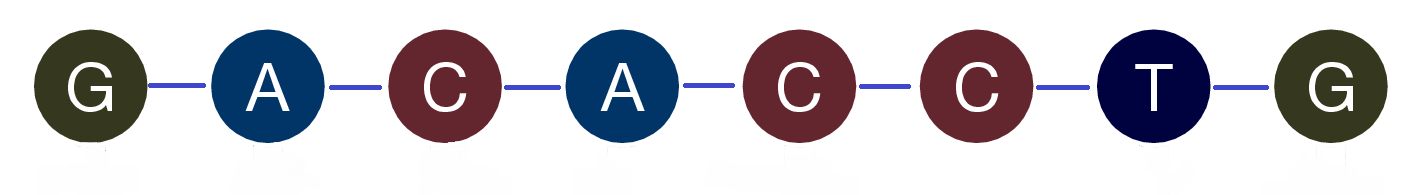
\includegraphics[width=.45\textwidth]{pictures/4.png}
    \end{center}
   
    \item Вторичная структура
    
    \begin{center}
    \vskip-20pt
    \hskip80pt
    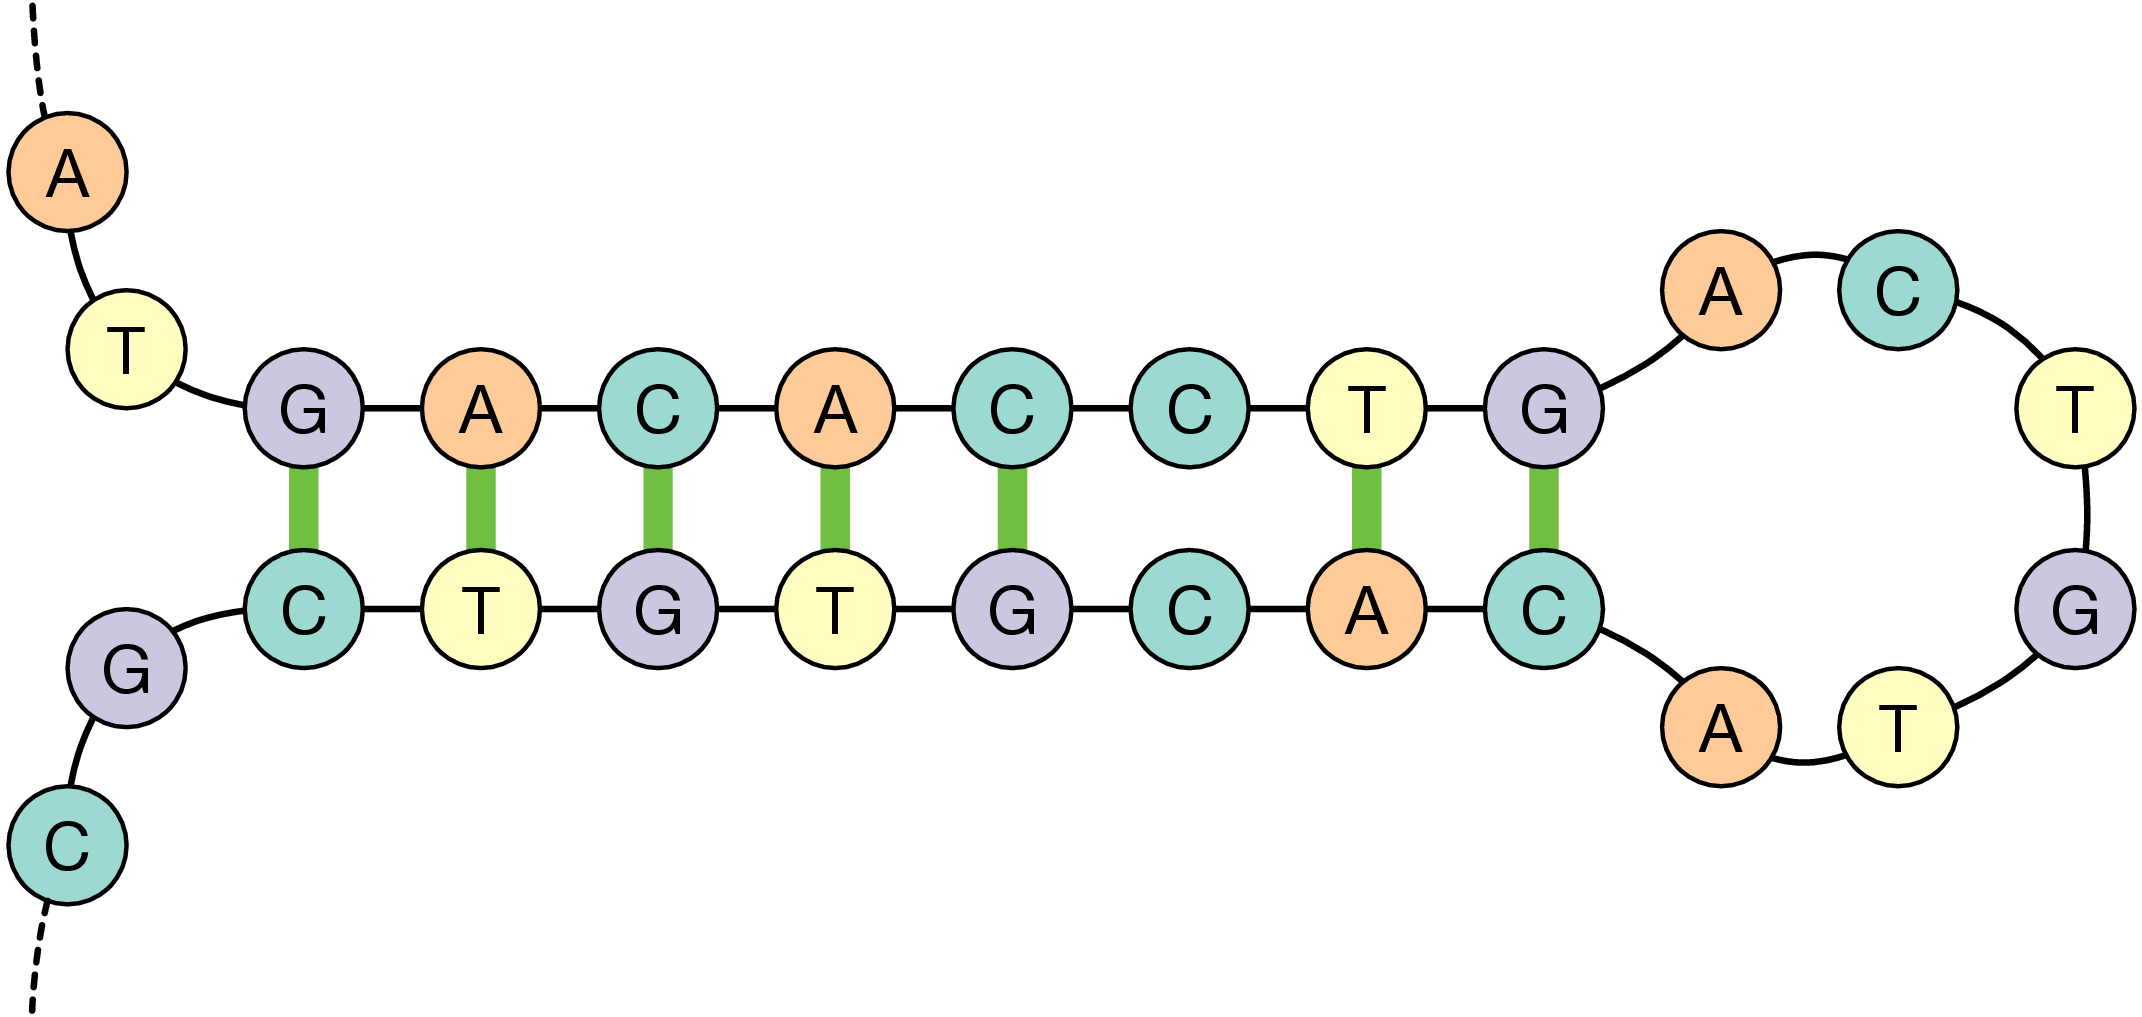
\includegraphics[width=.4\textwidth]{pictures/3.png}
    \end{center}
    
    %\begin{itemize}
    \item Особенности вторичной структуры существенны в задачах классификации и распознавания
    \item Вид вторичной структуры можно задать с помощью контекстно-свободной грамматики
    %\end{itemize}
    \end{itemize}
    
    
    \item \textbf {Задача:} поиск подстрок генетических цепочек, которые сворачиваются во вторичную структуру определенного вида
    \end{itemize}
    
\end{frame}


\begin{frame}
  \transwipe[direction=90]
  \frametitle{Алгоритмы синтаксического анализа}
    \begin{itemize}
    \item \textbf{Вход}:
    \begin{itemize}
    	\item $a_1...a_n$ --- строка
    	\item $G$ --- контекстно-свободная грамматика
    \end{itemize} 
    \item \textbf{Результат}: матрица разбора \textit{T}, элементы которой отвечают за выводимость конкретной подстроки из стартового нетерминала S ($a_{i+1}...a_{j} \in L_{G}(S) \Leftrightarrow S \in T[i,j]$)
    
    \end{itemize}
\end{frame}
            
\begin{frame}[fragile]
\transwipe[direction=90]
\frametitle{Алгоритм Валианта}
\begin{itemize}
\item Разбиение исходной матрицы и перемножение подматриц меньшего размера
\item Возможность расширения для других классов грамматик (конъюнктивных, булевых) 
\item Вычислительная сложность --- $\mathcal{O}(|G|BMM(n)\log{}n)$
    \begin{itemize}
        \item Матрица --- нетерминал
        \item $T[i,j] = \{ A \in N | T_A[i,j] = true\}$
    \end{itemize}
\end{itemize}

\begin{center}
\vskip-20pt
\hfill
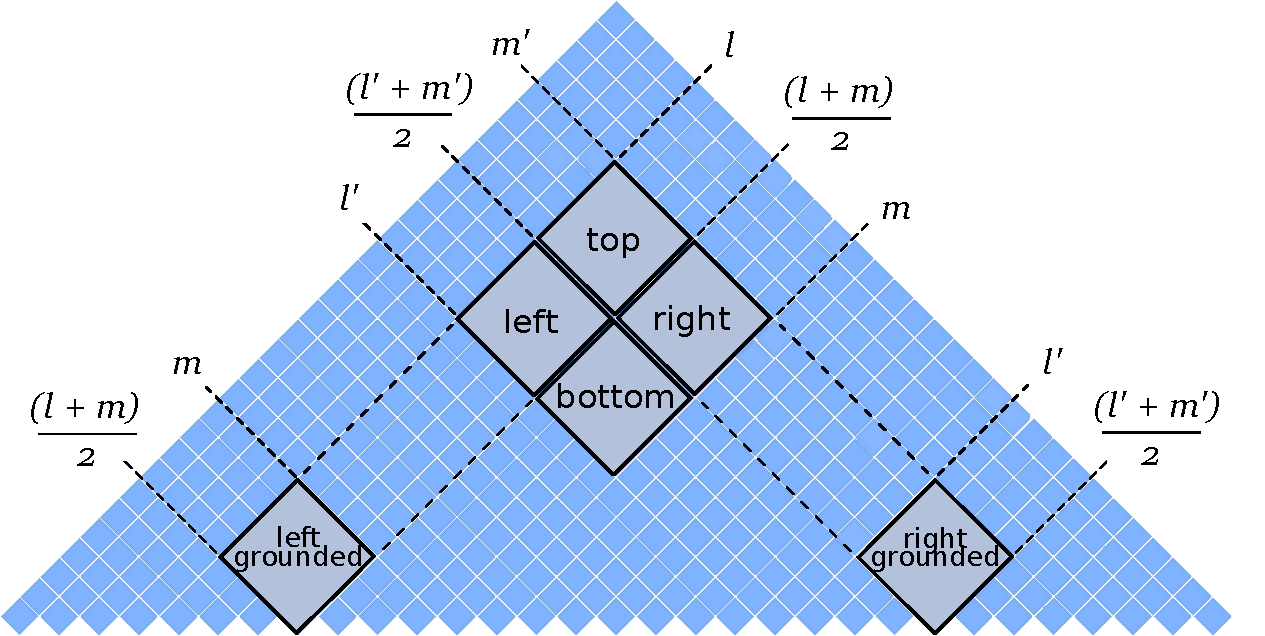
\includegraphics[width=.50\textwidth]{pictures/splitting_with_grounded.pdf}
\end{center}

\end{frame}


\begin{frame}[fragile]
  \transwipe[direction=90]
  \frametitle{Алгоритм Явейн}
    \\~
    \begin{itemize}
    \item Реогранизация вычислений
    \item Возможность разбиения на слои \linebreak подматриц
    \item Использование параллелизма на \linebreak уровне перемножения подматриц \linebreak слоя
    \end{itemize}
        \begin{center}
        \vskip-90pt \hskip190pt
        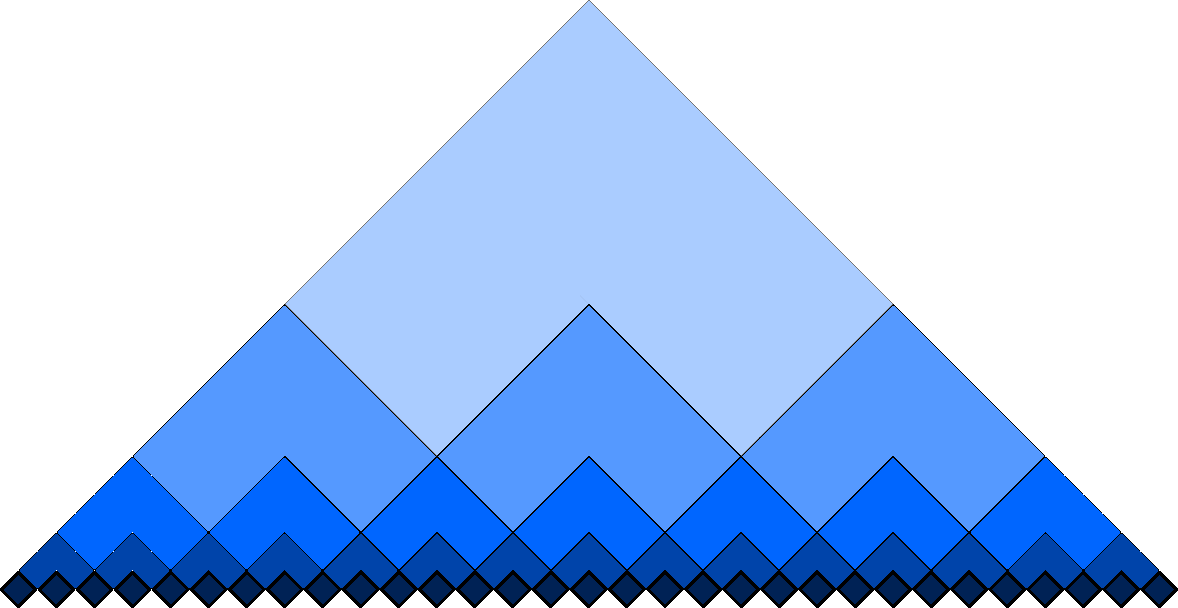
\includegraphics[width=.38\textwidth]{pictures/layers.pdf}
        \end{center} 

        \begin{center}
        \vskip5pt
        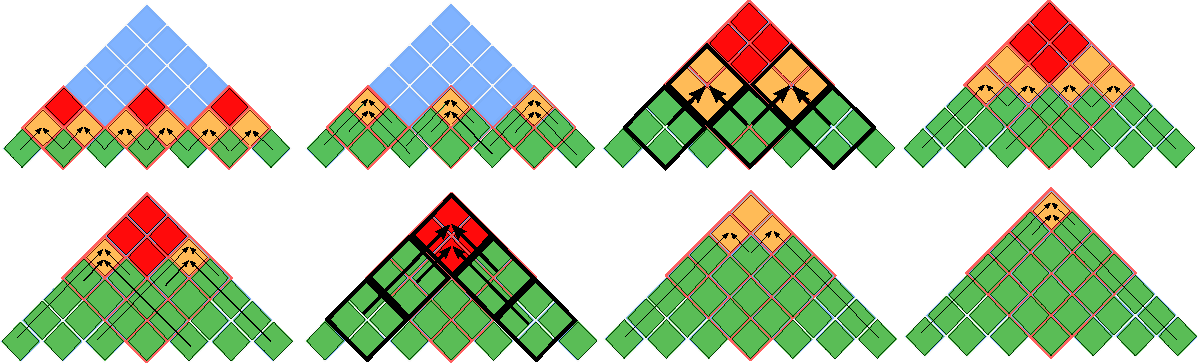
\includegraphics[width=.90\textwidth]{pictures/modivis_again.pdf} 
        \end{center} 
\end{frame}

\begin{frame}
\frametitle{Постановка задачи}
\textbf{Цель:} исследование алгоритма Явейн, являющегося модификацией алгоритма Валианта.
    
\vspace{5\onelineskip}
    
Для достижения данной цели были поставлены следующие задачи:
\begin{itemize}
	\item Доказать корректность алгоритма Явейн и дать оценку сложности
	\item Проанализировать эффективность применения этого алгоритма и алгоритма Валианта к задаче поиска подстрок
	\item Реализовать последовательную и параллельную версии алгоритмов Валианта и Явейн
	\item Выполнить экспериментальное исследование алгоритма Явейн
\end{itemize}
\end{frame}



\begin{frame}
  \transwipe[direction=90]
  \frametitle{Корректность алгоритма}
  \begin{rutheorem}[корректность алгоритма]
    Алгоритм Явейн корректно заполняет $T_{i, j}$ для всех i и j, и входная строка $a = a_{1}a_{2} \dots a_{n} \in L_{G}(S)$ тогда и только тогда, когда $S \in T_{0, n}$.

  \end{rutheorem}
\end{frame}

\begin{frame}
  \transwipe[direction=90]
  \frametitle{Оценка сложности алгоритма}
    \begin{rulemma}
     Для всех $ i \in \{ 1, .., p - 1\}$ матрицы размера $2^{p - i} \times 2^{p - i}$ перемножаются ровно $2^{2i - 1} - 2^{i}$ раз, где $n = 2^p - 1$ --- длина входной строки.
  \end{rulemma}
  
  \begin{rutheorem}[оценка сложность алгоритма]
    Пусть $|G|$ --- длина описания грамматики и \textit{n} --- длина входной строки. Тогда алгоритм Явейн заполняет матрицу \textit{T} за $\mathcal{O}(|G|BMM(n)\log{}n)$, где $BMM(n)$ --- время, необходимое для перемножения двух булевых матриц размера $n \times n$.
  \end{rutheorem}
  
\end{frame}

\begin{frame}
  \transwipe[direction=90]
  \frametitle{Применимость к задаче поиска подстрок}
  \begin{itemize}
      \item \textbf{Задача:} для входной строки размера $n = 2^p - 1$ найти все подстроки размера \textit{s}, которые принадлежат языку, заданному грамматикой
      \item \textbf{Алгоритм Валианта:} необходимо полностью вычислить, как минимум, две треугольные подматрицы размера $\frac{n}{2}$ $\mathcal{O}(|G|BMM(2^{p - 1})(p - 2))$
  \end{itemize}
  
  \begin{center}
  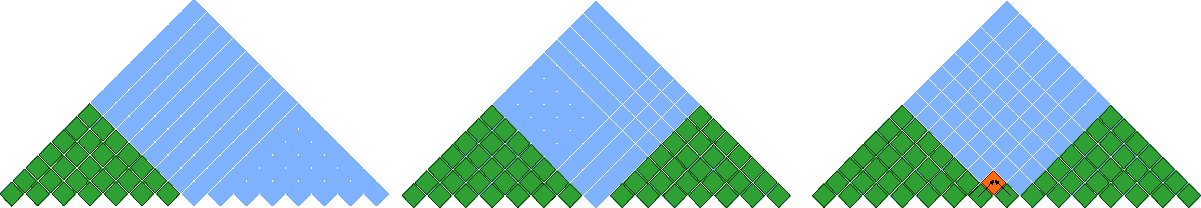
\includegraphics[width=.90\textwidth]{pictures/valsubstring.pdf}    
  \end{center}
  
  \begin{itemize}
      \item  \textbf{Алгоритм Явейн:} посчитать слои подматриц, размер которых не превышает $2^r$, где $2^{r-2} < s \le 2^{r - 1}$ \linebreak $\mathcal{O}(|G|2^{2(p - r) - 1}BMM(2^{r})(r - 1))$
  \end{itemize}
  
\end{frame}

\begin{frame}
  \transwipe[direction=90]
  \frametitle{Реализация}
  \begin{itemize}
    \item Реализация алгоритмов Валианта и Явейн
    \item Последовательная версия:
    \begin{itemize}
        \item Библиотека M4RI --- метод "четырех русских"
    \end{itemize}
    \item Параллельная версия:
    \begin{itemize}
        \item CUDA C
    \end{itemize}
    \end{itemize}
\end{frame}

\begin{frame}[fragile] \frametitle{Постановка экспериментов}
%\onslide<1-4>{

\begin{itemize}
    \item Грамматика D2

\small
\begin{alltt}
        s: s s | ( s ) | [ s ] | \varepsilon
\end{alltt}

\item Грамматика BIO

\small
\begin{alltt}
        s1: stem<s0>
        any_str: any_smb*[2..10]
        s0: any_str | any_str stem<s0> s0
        any_smb: A | T | C | G
        stem1<s>: A s T | G s C | T s A | C s G 
        stem2<s>: stem1<stem1<s>>
        stem<s>:  
              A stem<s> T 
            | T stem<s> A 
            | C stem<s> G 
            | G stem<s> C 
            | stem1<stem2<s>>  
\end{alltt}

\end{itemize}

\end{frame}




\begin{frame}{Эксперименты: сравнительный анализ}

\\~

    \begin{table*}
    \label{tbl1}
    \centering
    \resizebox{\columnwidth}{!}{%
    \begin{tabular}{|| c||c|c|c|c || c|c|c|c ||} 
    \hline
    \multirow{3}{*}{N} & \multicolumn{8}{c||}{Время (сек)} \\
    & \multicolumn{4}{c||}{Грамматика $D2$} & \multicolumn{4}{c||}{Грамматика $BIO$} \\
    & valCPU & yavCPU & valGPU & yavGPU & valCPU & yavCPU & valGPU & yavGPU   \\
    \hline
    127 & 0.08 & 0.08 & 0.20 & 0.10 & 1.35 & 1.34 & 0.19 & 0.10 \\
    255 & 0.28 & 0.30 & 0.52 & 0.13 & 5.40 & 5.50 & 0.53 & 0.14  \\
    511 & 1.21 & 1.18 & 1.90 & 0.25 & 21.97 & 22.35 & 1.99 & 0.26   \\
    1023 & 4.90 & 4.78 & 7.88 & 0.54 & 88.70 & 90.32 & 7.89 & 0.60  \\
    2047 & 19.61 & 19.38 & 33.50 & 1.50 & 363.32 & 374.20 & 34.01 & 1.70  \\
    4095 & 78.36 & 78.28 & 140.47 & 4.45 & 1467.68 & 1480.59 & 141.10 & 5.47 \\
    8191 & 315.67 & 315.08 & - & 13.65 & - & - & - & 18.04 \\
    \hline
    \end{tabular}
    }
    \end{table*}
    
    \vskip-10pt
    \begin{figure}[H]
    \centering
    \subfloat[]{
        \begin{tikzpicture}[scale=.40]
        \begin{axis}[
        legend cell align=left,
        legend pos = north west,
        xlabel = {Длина входной строки},
        ylabel = {Время, сек},
        label style={font=\Large}
        %ymode=log
        ]
        \addplot [color=blue, mark=triangle*] coordinates {
            (127, 0.078) (255, 0.289) (511,1.212) (1023,4.858) (2047,19.613) (4095,78.361)
        };
        \addplot [color=red, mark=*] coordinates {
            (127, 0.076) (255, 0.292) (511,1.177) (1023,4.779) (2047,19.379) (4095,78.279)
        };
        \legend{ 
            valCPU (D2), 
            yavCPU (D2)
        };
        \end{axis}
        \end{tikzpicture}
        \label{fig:GSSedges}
    }
        ~
    \subfloat[]{
        \begin{tikzpicture}[scale=.40]
        \begin{axis}[
        legend cell align=left,
        legend pos = north west,
        xlabel = {Длина входной строки},
        ylabel = {Время, сек},
        label style={font=\Large}
        %ymode=log
        ]
        \addplot [color=red, mark=triangle*] coordinates {
            (127, 0.078) (255, 0.289) (511,1.212) (1023,4.858) (2047,19.613) (4095,78.361)
        };
        \addplot [color=blue, mark=*] coordinates {
            (127, 1.345) (255, 5.408) (511,21.969) (1023,88.689) (2047,363.379) (4095,1467.675)
        };
        \legend{ 
            D2 (valCPU), 
            BIO (valCPU)
        };
        \end{axis}
        \end{tikzpicture}
        \label{fig:Time}
    }
    ~
    \subfloat[]{
        \begin{tikzpicture}[scale=.40]
        \begin{axis}[
        legend cell align=left,
        legend pos = north west,
        xlabel = {Длина входной строки},
        ylabel = {Время, сек},
        label style={font=\Large}
        %ymode=log
        ]
        \addplot [color=blue, mark=triangle*] coordinates {
            (127, 0.195) (255, 0.523) (511,1.995) (1023,7.888) (2047,34.008) (4095,141.173)
        };
        \addplot [color=red, mark=*] coordinates {
            (127, 0.105) (255, 0.140) (511,0.256) (1023,0.590) (2047,1.7) (4095,5.453)
        };
        \legend{ 
            valGPU (BIO), 
            yavGPU (BIO)
        };
        \end{axis}
        \end{tikzpicture}
        \label{fig:Time}
    }

    \label{expPlots}
\end{figure}


\end{frame}



\begin{frame}
\frametitle{Эксперименты: поиск подстрок}
    
    \begin{table*}
    
    \begin{center}
    \label{tbl3}
        \begin{tabular}{ ||c||c||c|c||c|c|| } 
        \hline
        \multirow{2}{*}{s}& \multirow{2}{*}{N} & \multicolumn{4}{c||}{Время (сек)}\\
        & & valCPU & yavCPU & valGPU & yavGPU \\
        \hline
        \multirow{4}{*}{250} & 1023 & 4.90 & 3.00 & 7.88 & 0.24 \\ 
        & 2047 & 19.61 & 6.65 & 33.50 & 0.26\\ 
        & 4095 & 78.36 & 13.83 & 140.47 & 0.32\\ 
        & 8191 & 315.67 & 28.90 & - & 0.46\\ 
        \hline
        \multirow{3}{*}{510} & 2047 & 19.61 & 12.18 & 33.50 & 0.58\\
        & 4095 & 78.36 & 26.58 & 140.47 & 0.65\\
        & 8191 & 315.67 & 56.70 & -  & 0.88\\ 
        \hline
        \multirow{2}{*}{1020} & 4095 & 78.36 & 48.31 & 140.47 & 1.59 \\
        & 8191 & 315.67 & 108.38 & - & 1.95\\ 
        \hline
        2040 & 8191 & 315.67 & 197.32 & - & 5.10\\ 
        \hline
        \end{tabular}
    \end{center}
    
    \end{table*}

\end{frame}



\begin{frame}
  \transwipe[direction=90]
  \frametitle{Результаты}
  \begin{itemize}
	\item Доказана корректность алгоритма Явейн и дана оценка вычислительной сложности, которая составляет $\mathcal{O}(|G|BMM(n)log(n))$
	\item Проведен анализ, который показал, что алгоритм Явейн лучше применим к задаче поиска подстрок, чем оригинальная версия алгоритма
	\item Реализованы последовательная и параллельная версии алгоритмов Валианта и Явейн. Исходный код доступен в репозитории: https://github.com/SusaninaJulia/PBMM
	\item Проведено экспериментальное исследование алгоритма Явейн, показавшее его эффективность  
	\item Результаты работы приняты к публикации в журнале <<Труды ИСП РАН>>
    \end{itemize}
\end{frame}

\end{document}
